\documentclass{article}
\usepackage{amsmath}
\usepackage{amssymb}
\usepackage{graphicx}
\usepackage[margin=1in]{geometry}
\usepackage{hyperref}
\usepackage{caption}
\usepackage{float}
\graphicspath{{images/}}
\hypersetup{
    colorlinks=true,
    urlcolor=blue,
}
\begin{document}

\title{The World Record Quartic}
\author{Aresh Pourkavoos}
\maketitle

I recently watched \href{https://youtu.be/UVfR9u1TGW0}{this Tibees video} on algebraic surfaces
and got inspired to experiment with them on my own using the SURFER program.
Please watch it before continuing, as I will reference it.

The equation for the Barth sextic given in the video, with a bit of my own modification, is
$$4(\varphi^2x^2-y^2)(\varphi^2y^2-z^2)(\varphi^2z^2-x^2)-\varphi^3(x^2+y^2+z^2-1)^2=0,$$
where $\varphi$ is the golden ratio.
Tibees mentions that the first term is the product of six planes,
which can be seen by separating each factor using the difference of two squares,
e.g. $\varphi^2x^2-y^2 = (\varphi x+y)(\varphi x-y)$.
Each of these binomial terms is 0 at all points on some plane passing through the origin,
which is perpendicular to some vector.
The previous binomials, for example, represent planes
perpendicular to $(\varphi, 1, 0)$ and $(\varphi, -1, 0)$, respectively.
Separating the other two quadratic factors in the same way yields
six planes and six perpendicular vectors.
Taking the negative of each vector (which is perpendicular to the same plane)
produces 12 vectors in total, which form the vertices of an icosahedron.
The planes themselves, when projected onto a sphere centered at the origin,
become great circles which trace out the edges of an icosidodecahedron.

\begin{center}
  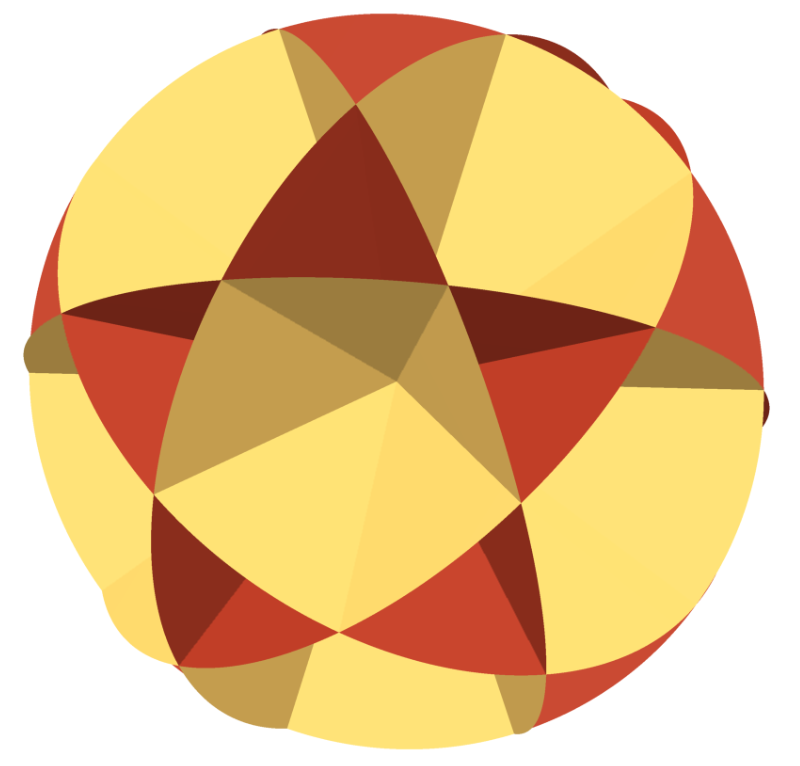
\includegraphics[width=0.25\linewidth]{id.png}
\end{center}
I knew of a similar relationship between polyhedra,
where the vertices of one become the equators of another: the cube and the cuboctahedron.
In this case, the 8 vertices of the cube generate 4 planes:
$x+y+z=0$, $x+y-z=0$, $x-y+z=0$, and $x-y-z=0$.
\begin{center}
  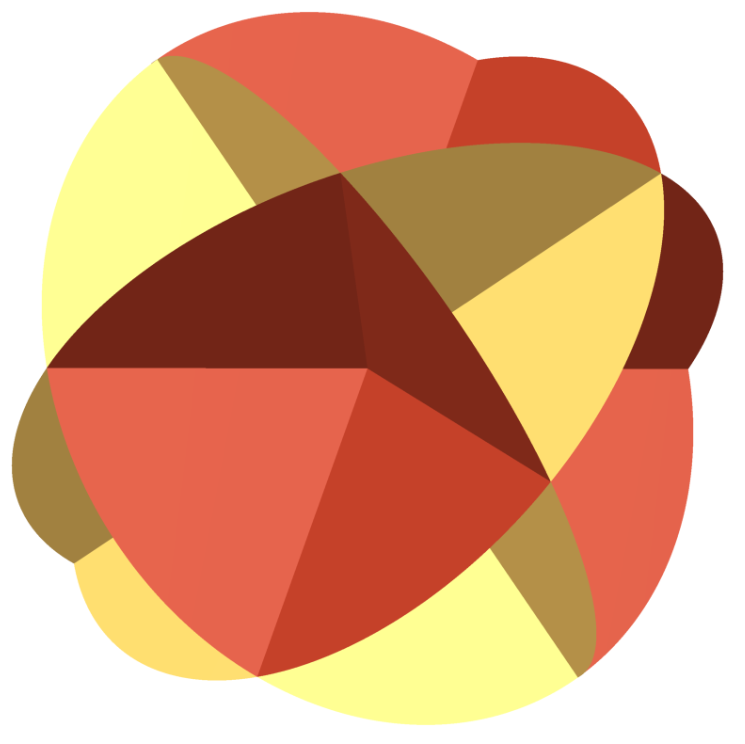
\includegraphics[width=0.25\linewidth]{co.png}
\end{center}
In SURFER, I simply replaced the first term in the Barth sextic with the product of these planes
and the $\varphi^3$ with a variable $a$ to obtain
$$(x+y+z)(x+y-z)(x-y+z)(x-y-z)-a(x^2+y^2+z^2-1)^2=0,$$
where $a$ could be adjusted via a slider.
As predicted, there appeared to be twelve singularities at the vertices of the cuboctahedron
regardless of the value of $a$.
However, I still had to verify them with the mathematical definition of a singularity.
As Tibees says, they are points where the partial derivatives vanish (i.e. equal zero),
so I computed these for $f(x, y, z)$, the left side of the equation of the surface:
\begin{align*}
  \frac{\partial f}{\partial x} &= 4x(x^2-y^2-z^2-a(x^2+y^2+z^2-1)) \\
  \frac{\partial f}{\partial y} &= 4y(y^2-x^2-z^2-a(x^2+y^2+z^2-1)) \\
  \frac{\partial f}{\partial z} &= 4z(z^2-x^2-y^2-a(x^2+y^2+z^2-1))
\end{align*}
All of these must be zero, in addition to $f(x, y, z)$ itself,
for $(x, y, z)$ to be considered a singularity.
I found that the singularities occurred at
$\left(0, \pm\frac{1}{\sqrt{2}}, \pm\frac{1}{\sqrt{2}}\right)$,
$\left(\pm\frac{1}{\sqrt{2}}, 0, \pm\frac{1}{\sqrt{2}}\right)$, and
$\left(\pm\frac{1}{\sqrt{2}}, \pm\frac{1}{\sqrt{2}}, 0\right)$,
which form the vertices of a cuboctahedron of edge length 1.
More briefly, the singularities occur at all permutations and sign changes of
$\left(0, \frac{1}{\sqrt{2}}, \frac{1}{\sqrt{2}}\right)$.
Since the slider for $a$ ran from 0 to 1, it didn't take long for me to find $a=1$,
which generated this surface.
\begin{center}
  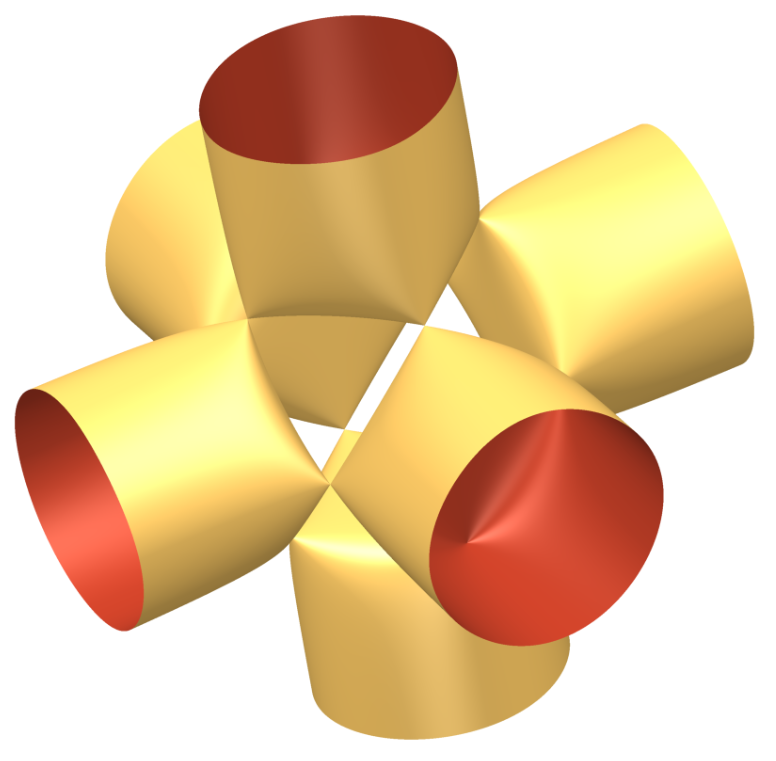
\includegraphics[width=0.25\linewidth]{co2.png}
\end{center}
The six squares of the cuboctahedron extend into three pairs of cylinders,
and I suspected that in addition to the twelve singularities I had already verified,
there were three at the points at infinity in the direction of these cylinders, for a total of 15.
The video also shows that the maximum number of singularities for a quartic is 16,
and further research reveals that the world record is held by the Kummer surface.

(Image)

Since my surface with 15 singularities was tantalizingly close to the maximum possible 16,
I wondered if values of $a$ outside the initial range would allow me to tie the world record.
Sure enough, $a=-\frac{1}{3}$ produced this surface,
with the eight triangles extending into four pairs of cylinders,
supposedly creating four singularities at infinity.
\begin{center}
  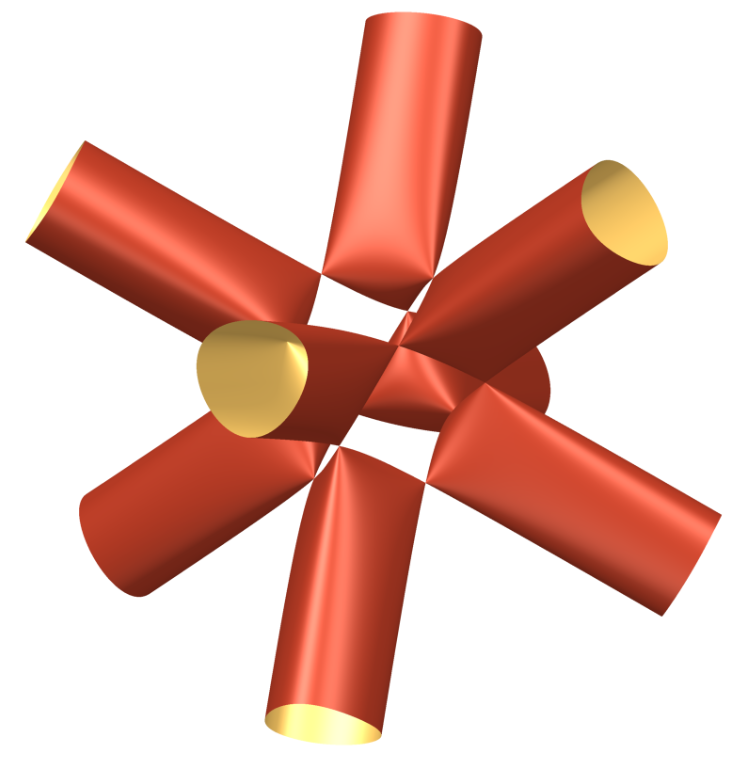
\includegraphics[width=0.25\linewidth]{co3.png}
\end{center}
To put the singularities at the permutations and sign changes of $(0, 1, 1)$ for aesthetics,
I decided to scale up the surface by a factor of $\sqrt{2}$
and rearrange the equation:
$$3(x^4+y^4+z^4+1)-(x^2+y^2+z^2+1)^2=0$$

To verify this intuition about the points at infinity, though,
I had to construct the surface in projective space,
which is defined in 4D rather than 3D.
Points in projective 3D space ($\mathbb{P}^3$)
are defined as lines passing through the origin in 4D space ($\mathbb{R}^4$),
or equivalently, as the multiples of some non-null vector $(x, y, z, w)$.
To recover the point in 3D, intersect the line in 4D with the hyperplane $w=1$,
or equivalently, divide the other three coordinates by $w$
to get $\left(\frac{x}{w}, \frac{y}{w}, \frac{z}{w}\right)$.
If $w\neq0$, this division works as usual, and the result is a point in $\mathbb{R}^3$.
If $w=0$, however, the line in 4D does not intersect the hyperplane $w=1$ at all,
and the division does not return a real number.
The line, however, still represents some point in $\mathbb{P}^3$,
which is known as a point at infinity.

To rewrite the equation of an algebraic surface in projective space,
replace $x$, $y$, and $z$ with $\frac{x}{w}$, $\frac{y}{w}$, and $\frac{z}{w}$, respectively,
and multiply by the appropriate power of $w$ to get rid of the denominators.
For example,

(Example)

Note that the same equation can be reached by multiplying all of the lower-degree terms by $w$
until they reach the highest degree of any term in the polynomial.
Applying this method to the surface I had found, I obtained
$$3(x^4+y^4+z^4+w^4)-(x^2+y^2+z^2+w^2)^2=0$$
and was pleasantly surprised to see that it was symmetrical in all four variables!
I could have used these symmetries to find the singularities at the points at infinity,
but I decided to repeat the process
and take the partial derivatives of this function $g(x, y, z, w)$:
\begin{align*}
  \frac{\partial g}{\partial x} &= 4x(2x^2-y^2-z^2-w^2) \\ 
  \frac{\partial g}{\partial y} &= 4y(2y^2-x^2-z^2-w^2) \\ 
  \frac{\partial g}{\partial z} &= 4z(2z^2-x^2-y^2-w^2) \\ 
  \frac{\partial g}{\partial w} &= 4w(2w^2-x^2-y^2-z^2) 
\end{align*}
Setting these and $g$ itself equal to zero revealed the singularities as lines in 4D:
the permutations and sign changes of $(0, c, c, c)$ for any constant $c$.
At first glance, it appears that 4 permutations and $2^3=8$ sign changes would yield 32 lines,
but in reality, there are only 4 sign changes, as negating all $c$s creates the same line again.
If, however, you take a given point on one of these lines, say $(0, 1, 1, 1)$,
and apply all 32 transformations, the resulting 4D shape is a rectified tesseract:

\begin{center}
  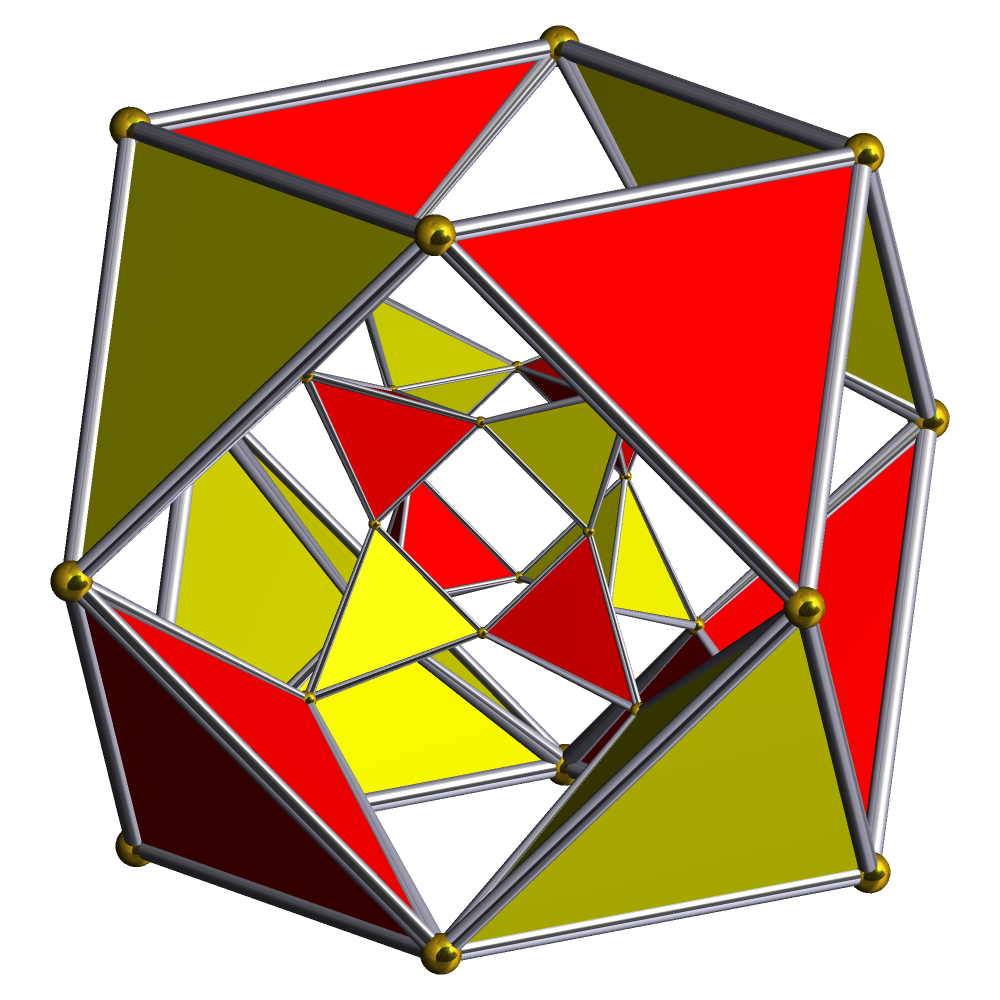
\includegraphics[width=0.25\linewidth]{rit.png}
\end{center}
It has 24 3D cells: 16 tetrahedra and 8 cuboctahedra,
positioned around the vertices and cells of a tesseract, respectively.
In the original 3D surface, we can clearly see a cuboctahedron in the center,
and the eight cylinders adjacent to it are actually tetrahedra
whose fourth vertices reside at infinity.
There are also six half-cuboctahedra connecting to the square faces in the center,
but they are extremely distorted and hard to see.
Since the surface is a projection of half of a rectified tesseract,
I wanted to see whether it was possible to transform it
to obtain a projection of the full shape.

$$3(x^4+y^4+z^4+(x^2+y^2+z^2-1)^4)-(x^2+y^2+z^2+(x^2+y^2+z^2-1)^2)^2 = 0$$

\begin{align*}
  m &= x^2 \\
  n &= y^2 \\
  p &= z^2 \\
  q &= w^2 \\
  l_1 &= m^2+n^2+p^2+q^2 \\
  l_2 &= mn+pq \\
  l_3 &= mp+nq \\
  l_4 &= mq+pn \\
  l_5 &= mnpq \\
  s_{1,0} &= l_1(l_2l_3+l_2l_4+l_3l_4) \\
  s_{1,1} &= l_1^2(l_2+l_3+l_4) \\
  s_{1,2} &= l_1(l_2^2+l_3^2+l_4^2) \\
  s_{5,1} &= l_5(l_2+l_3+l_4) \\
  s_{2,3,4} &= l_2^3+l_3^3+l_4^3 \\
  s_{2,3}^{\pm} &= l_2^2l_3 \pm l_2l_3^2 \\
  s_{3,4}^{\pm} &= l_3^2l_4 \pm l_3l_4^2 \\
  s_{4,2}^{\pm} &= l_4^2l_2 \pm l_4l_2^2 \\
  Q_{12} &= (m+n+p+q)^6 \\
  S_{12} &= 33\sqrt{5}(s_{2,3}^{-}+s_{3,4}^{-}+s_{4,2}^{-})+19(s_{2,3}^{+}+s_{3,4}^{+}+s_{4,2}^{+}) \\
  &+ 10s_{2,3,4}-14s_{1,0}+2s_{1,1}-6s_{1,2}-352s_{5,1}+336l_5^2l_1+48l_2l_3l_4 \\
  X_{12} &= 243S_{12}-22Q_{12}=0
\end{align*}

\end{document}
